\chapter{Mathematical Formulations}
\label{chap:mathematical_formulations}
\section{Softmax}
\label{sec:softmax}
We can use the softmax function to transfer the model scores to probabilities for a multi-class classification problem. For further reference on the softmax implementation, see \cite{https://doi.org/10.48550/arxiv.1704.00805} as:
\begin{equation}
    \label{eqn:softmax}
    \sigma_i(\hat{y}):=\frac{\exp(\hat{y}_i)}{\sum_{j=1}^{d}\exp(\hat{y}_j)}, 1\leq i \leq n
\end{equation}
where $d$ is the number of classes and $i$ indicating the current pixel. The function applies a pointwise exponential and divides it by the sum over the exponential as a normalization to ensure that all components sum up to one. \figref{predictions_scores_softmax} depicts the transformation of an output score to an output with probabilities using the softmax function.

\begin{figure}[H]%[htbp]
    \centering
    \subfigure[]{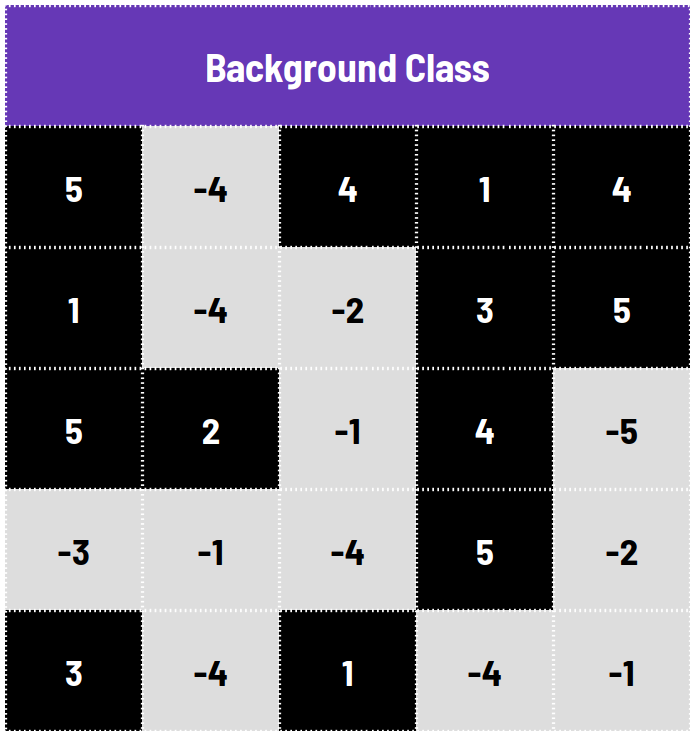
\includegraphics[width=\imgWidthFour]{images/predictions_scores_softmax_4.png}}
    \subfigure[]{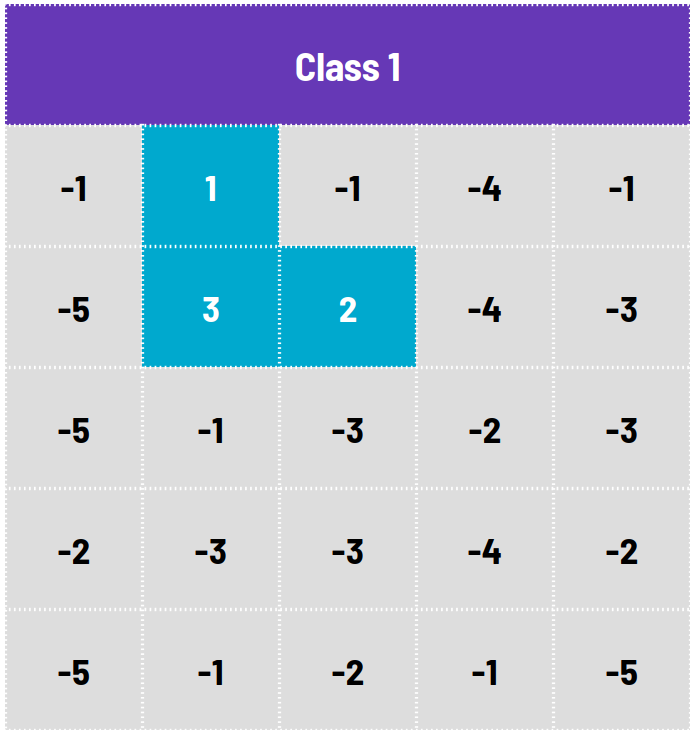
\includegraphics[width=\imgWidthFour]{images/predictions_scores_softmax_1.png}}
    \subfigure[]{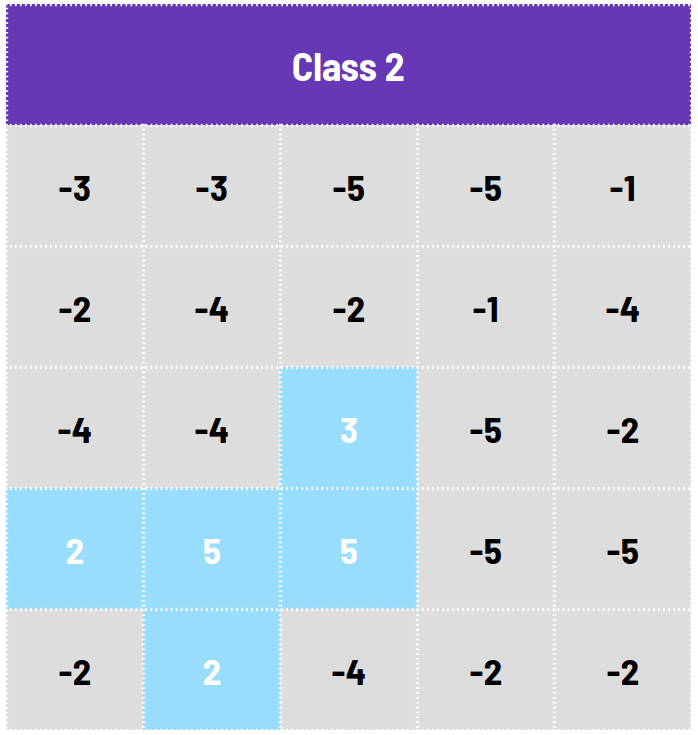
\includegraphics[width=\imgWidthFour]{images/predictions_scores_softmax_2.png}}
    \subfigure[]{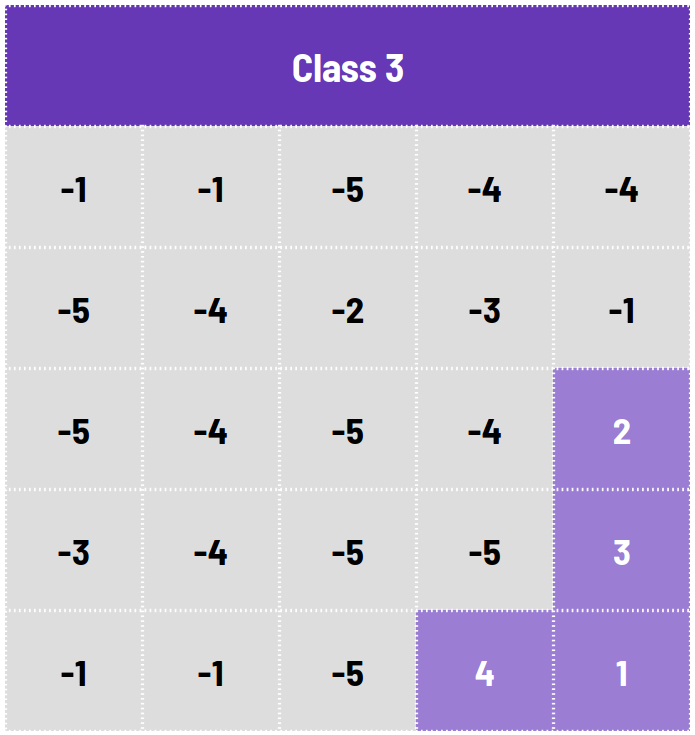
\includegraphics[width=\imgWidthFour]{images/predictions_scores_softmax_3.png}}\\
    \subfigure[]{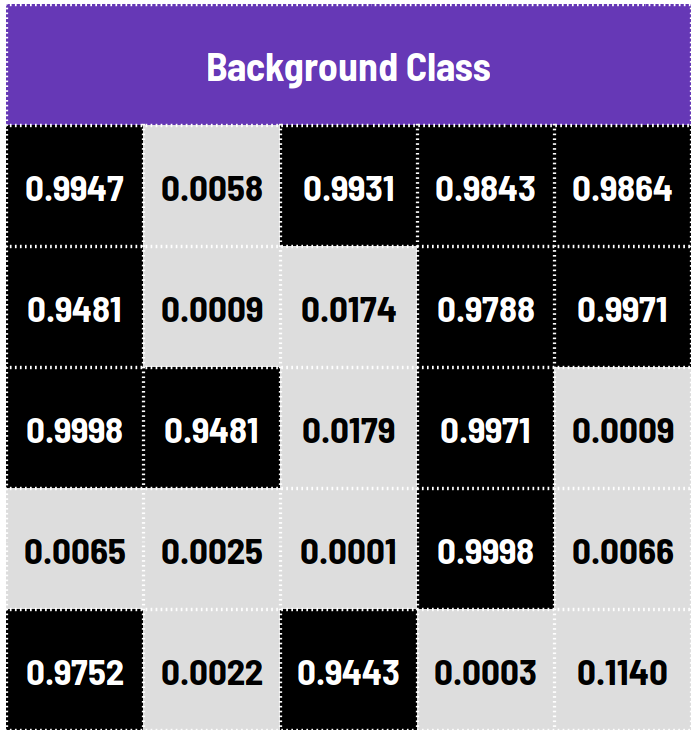
\includegraphics[width=\imgWidthFour]{images/predictions_scores_softmax_8.png}}
    \subfigure[]{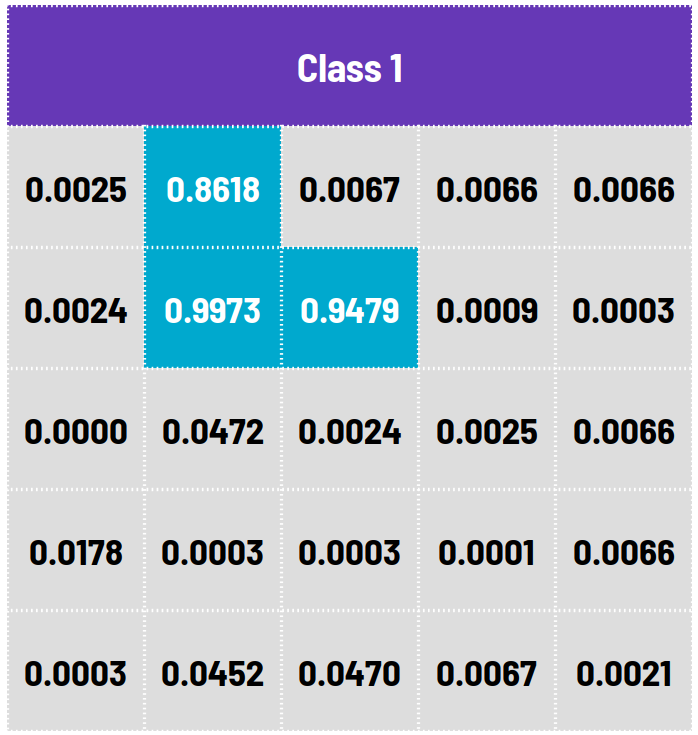
\includegraphics[width=\imgWidthFour]{images/predictions_scores_softmax_5.png}}
    \subfigure[]{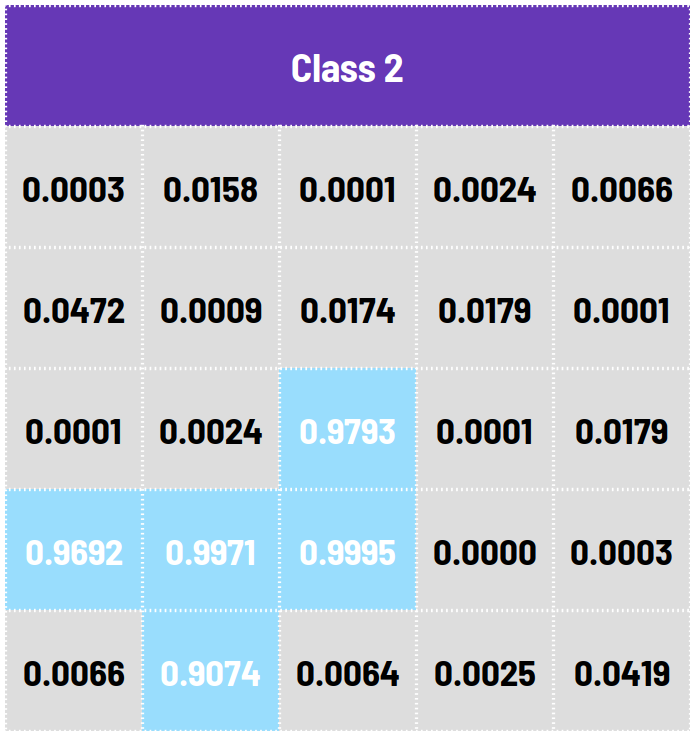
\includegraphics[width=\imgWidthFour]{images/predictions_scores_softmax_6.png}}
    \subfigure[]{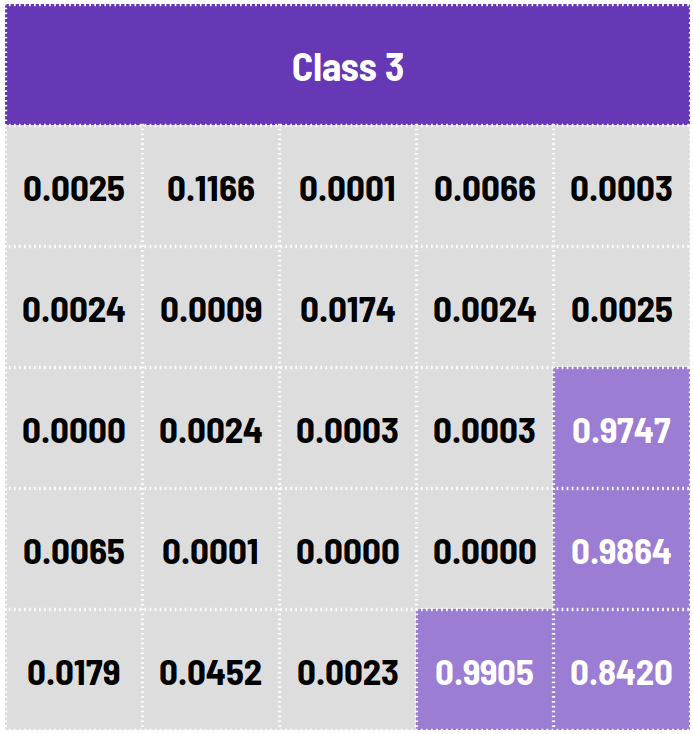
\includegraphics[width=\imgWidthFour]{images/predictions_scores_softmax_7.png}}
    \caption[Scores $\to$ probabilities]{(a-d) Output from \ac{CNN} with scores transferred to probabilities (e-h) with equation \ref{eqn:softmax}}
    \label{predictions_scores_softmax}
\end{figure}